% ================= IF YOU HAVE QUESTIONS =======================
%
% Technical questions to bbob@lri.fr
% ===============================================================
%
\documentclass{article}
%%%%%%%%%%%%%%%%%%%%%%%%%%%%% PREAMBLE   %%%%%%%%%%%%%%%%%%%%%%%%%%%%%%%%%%%%%%
\usepackage{amssymb,amsmath}
%\usepackage{wasysym} % needed for some symbols varhexagon hexagon pentagon
%\usepackage{MnSymbol} % needed for some other symbols upY downY leftY rightY
\usepackage{xstring} % for string operations
\usepackage{graphicx}
\usepackage{float}
\usepackage{rotating}
\usepackage{lscape}
\usepackage{colortbl}
\usepackage[table]{xcolor}
\usepackage{tabularx}
\definecolor{tableShade}{HTML}{ECF3FE}
\newcommand{\DIM}{\ensuremath{\mathrm{DIM}}}
\newcommand{\ERT}{\ensuremath{\mathrm{ERT}}}
\newcommand{\FEvals}{\ensuremath{\mathrm{FEvals}}}
\newcommand{\nruns}{\ensuremath{\mathrm{Nruns}}}
\newcommand{\Dfb}{\ensuremath{\Delta f_{\mathrm{best}}}}
\newcommand{\Df}{\ensuremath{\Delta f}}
\newcommand{\nbFEs}{\ensuremath{\mathrm{\#FEs}}}
\newcommand{\fopt}{\ensuremath{f_\mathrm{opt}}}
\newcommand{\ftarget}{\ensuremath{f_\mathrm{t}}}
\newcommand{\CrE}{\ensuremath{\mathrm{CrE}}}
\newcommand{\tablecaption}[2]{\ERT\ on $f_{#1}$ in #2-D over \ERT$_\text{best}$
obtained in BBOB 2009}
%%%%%%%%%%%%%%%%%%%%   END OF PREAMBLE   %%%%%%%%%%%%%%%%%%%%%%%%%%%%%%%%%%%%%%
% \newcommand{\bbobdatapath}{ppdatamany/} % was default output folder of rungenericmany.py 
\newcommand{\bbobdatapath}{ppdata/} % default output folder of rungeneric.py

\input{\bbobdatapath bbob_pproc_commands.tex}
\graphicspath{{\bbobdatapath}}

\title{Black-Box Optimization Benchmarking Template for the Comparison of Algorithms on the Noiseless Testbed}
\author{}

\begin{document}

\maketitle

% \section{Introduction}
%
% \section{Algorithm Presentation}
%
% \section{Experimental Procedure}
%
%%%%%%%%%%%%%%%%%%%%%%%%%%%%%%%%%%%%%%%%%%%%%%%%%%%%%%%%%%%%%%%%%%%%%%%%%%%%%%%
\section{Results}
%%%%%%%%%%%%%%%%%%%%%%%%%%%%%%%%%%%%%%%%%%%%%%%%%%%%%%%%%%%%%%%%%%%%%%%%%%%%%%%
Results from experiments according to \cite{hansen2010exp} on the benchmark
functions given in \cite{wp200901_2010,hansen2010fun} are presented in 
Figures~\ref{fig:scaling}, \ref{fig:ECDFs05D} and \ref{fig:ECDFs20D}.
The \textbf{expected running time (\ERT)}, used in the figures and table,
depends on a given target function value, $\ftarget=\fopt+\Df$, and is computed
over all relevant trials as the number of function evaluations executed during
each trial while the best function value did not reach \ftarget, summed over
all trials and divided by the number of trials that actually reached \ftarget\
\cite{hansen2010exp,price1997dev}.
\textbf{Statistical significance} is tested with the rank-sum test for a given
target $\Delta\ftarget$ using, for each trial, either the number of needed
function evaluations to reach $\Delta\ftarget$ (inverted and multiplied by
$-1$), or, if the target was not reached, the best $\Df$-value achieved,
measured only up to the smallest number of overall function evaluations for any
unsuccessful trial under consideration if available.
Tables~\ref{tab:f1_05D} to \ref{tab:f24_05D} and \ref{tab:f1_20D} to \ref{tab:f24_20D}
give the Expected Running Time (\ERT) for targets $10^{1,\,-1,\,-3,\,-5,\,-7}$
divided by the best \ERT\ obtained during BBOB-2009 (given in the
\ERT$_{\text{best}}$ row), respectively in 5-D and 20-D.
Bold entries correspond to the best (or 3-best if there are more than 3
algorithms) values.
The median number of conducted function evaluations is additionally given in
\textit{italics}, if $\ERT(10^{-7}) =\infty$.
\#succ is the number of trials that reached the final target $\fopt + 10^{-8}$.
Entries with the $\downarrow$ symbol are statistically significantly better 
(according to the rank-sum test) compared to the best algorithm in BBOB-2009,
with $p=0.05$ or $p=10^{-k}$ where $k>1$ is the number
following the $\downarrow$ symbol, with Bonferroni correction of 24.
%%%%%%%%%%%%%%%%%%%%%%%%%%%%%%%%%%%%%%%%%%%%%%%%%%%%%%%%%%%%%%%%%%%%%%%%%%%%%%%
%%%%%%%%%%%%%%%%%%%%%%%%%%%%%%%%%%%%%%%%%%%%%%%%%%%%%%%%%%%%%%%%%%%%%%%%%%%%%%%
\begin{figure}
\centering
\begin{tabular}{@{}c@{}c@{}c@{}c@{}}
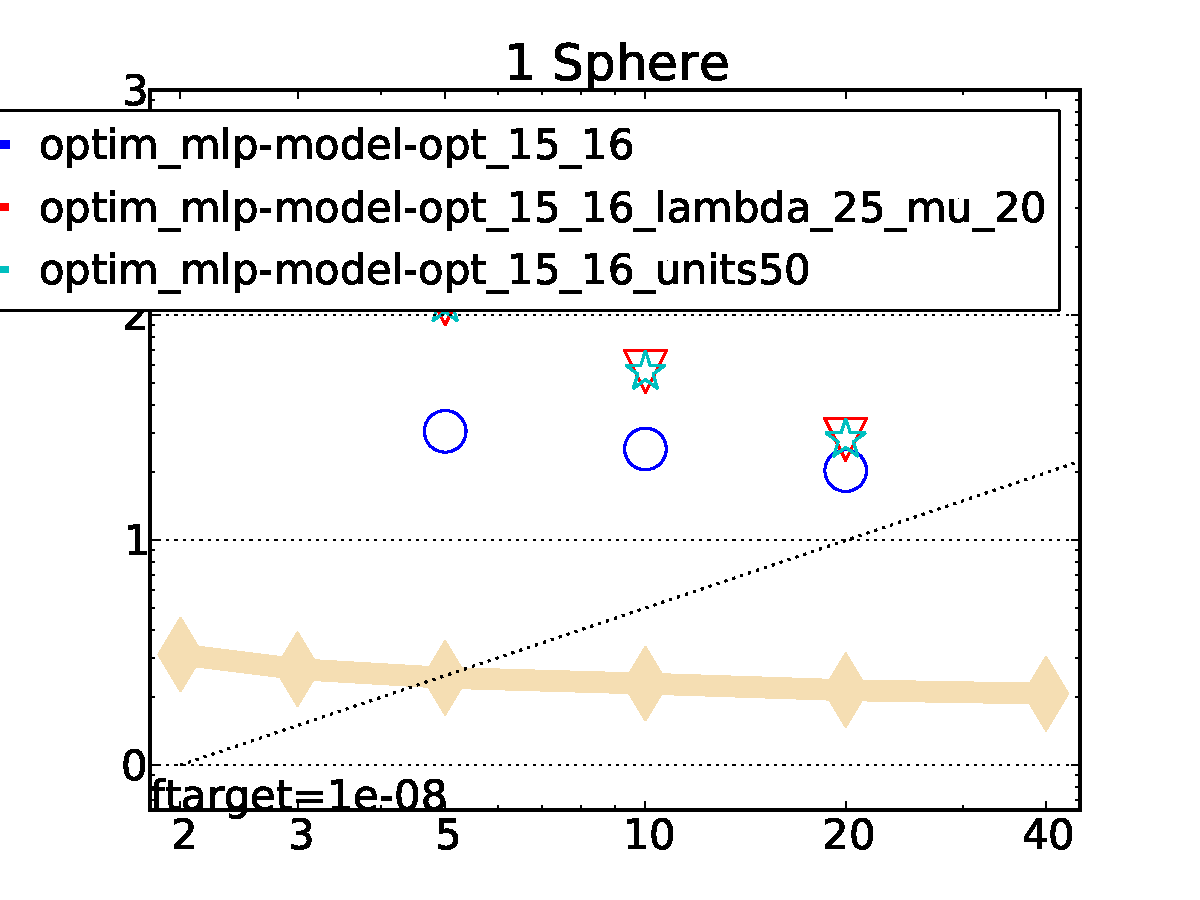
\includegraphics[width=0.25\textwidth, trim=20mm 7mm 15mm 3mm, clip]{ppfigs_f001}&
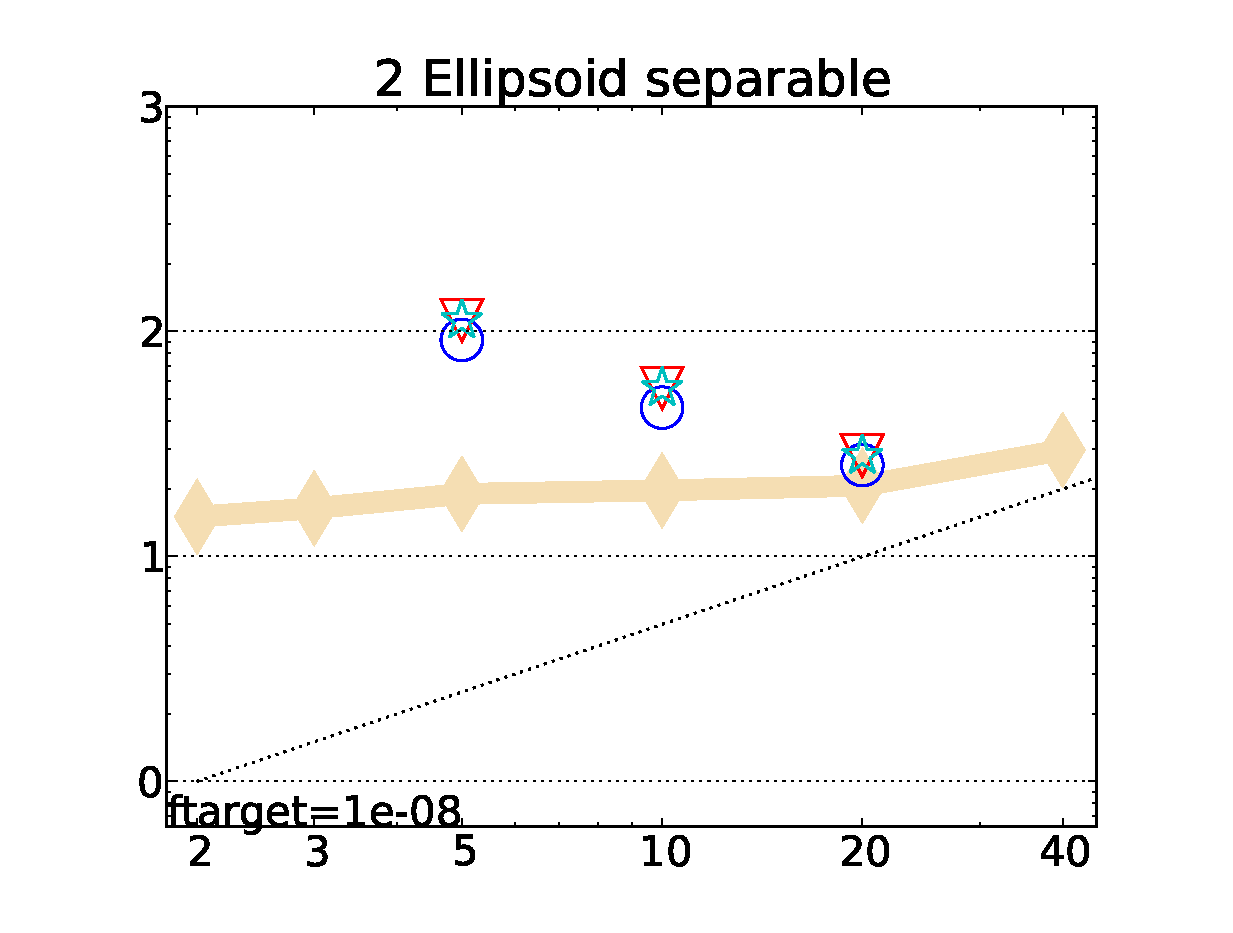
\includegraphics[width=0.25\textwidth, trim=20mm 7mm 15mm 3mm, clip]{ppfigs_f002}&
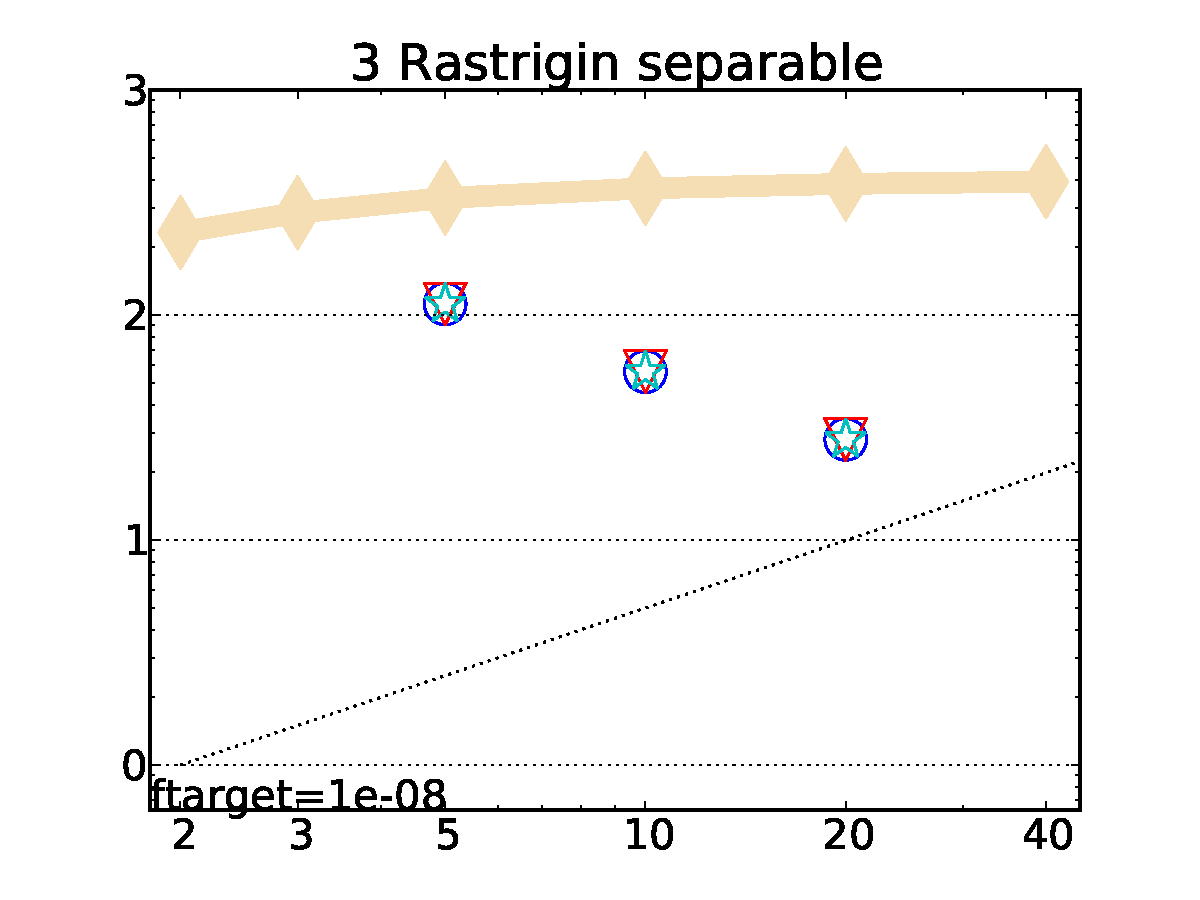
\includegraphics[width=0.25\textwidth, trim=20mm 7mm 15mm 3mm, clip]{ppfigs_f003}&
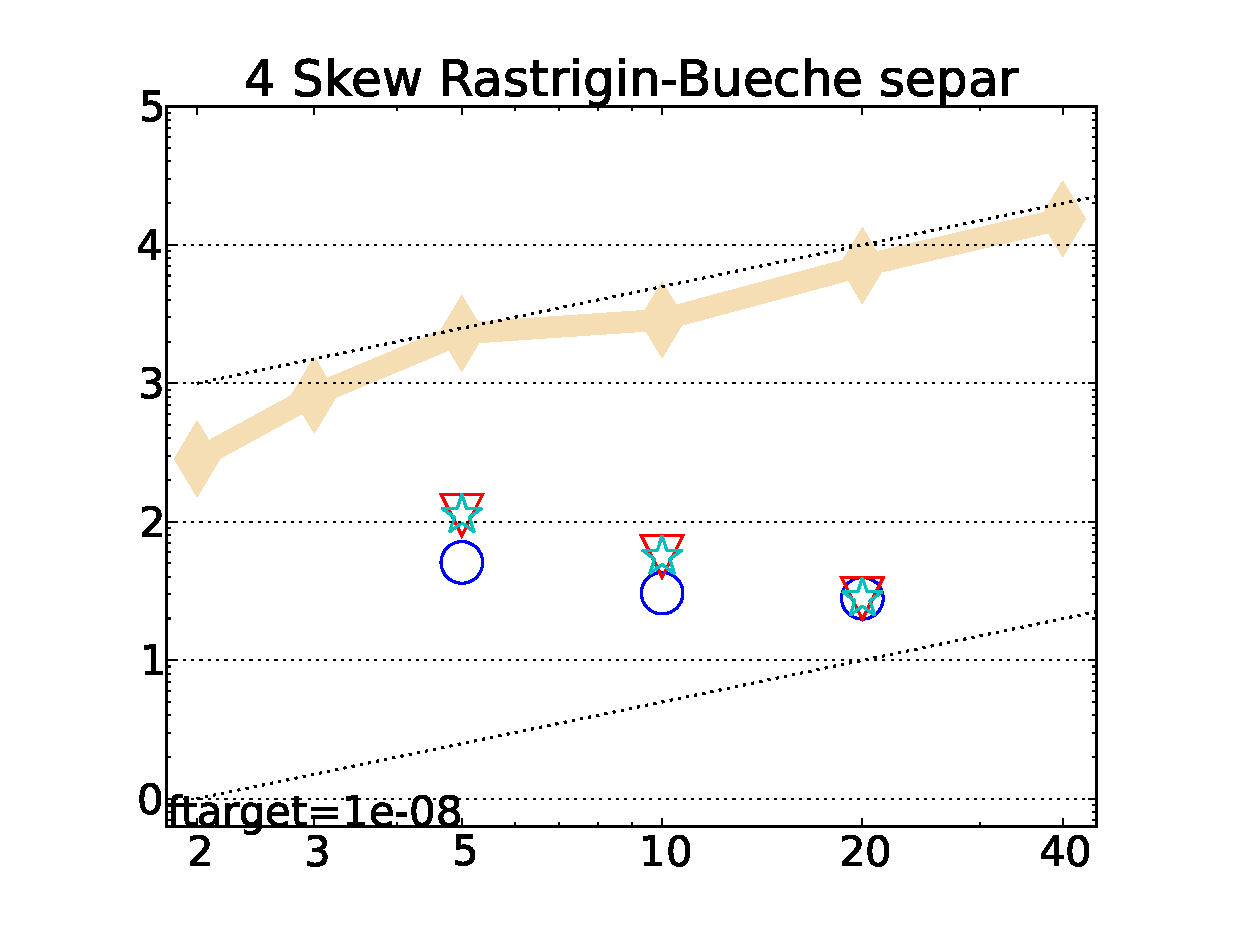
\includegraphics[width=0.25\textwidth, trim=20mm 7mm 15mm 3mm, clip]{ppfigs_f004}\\
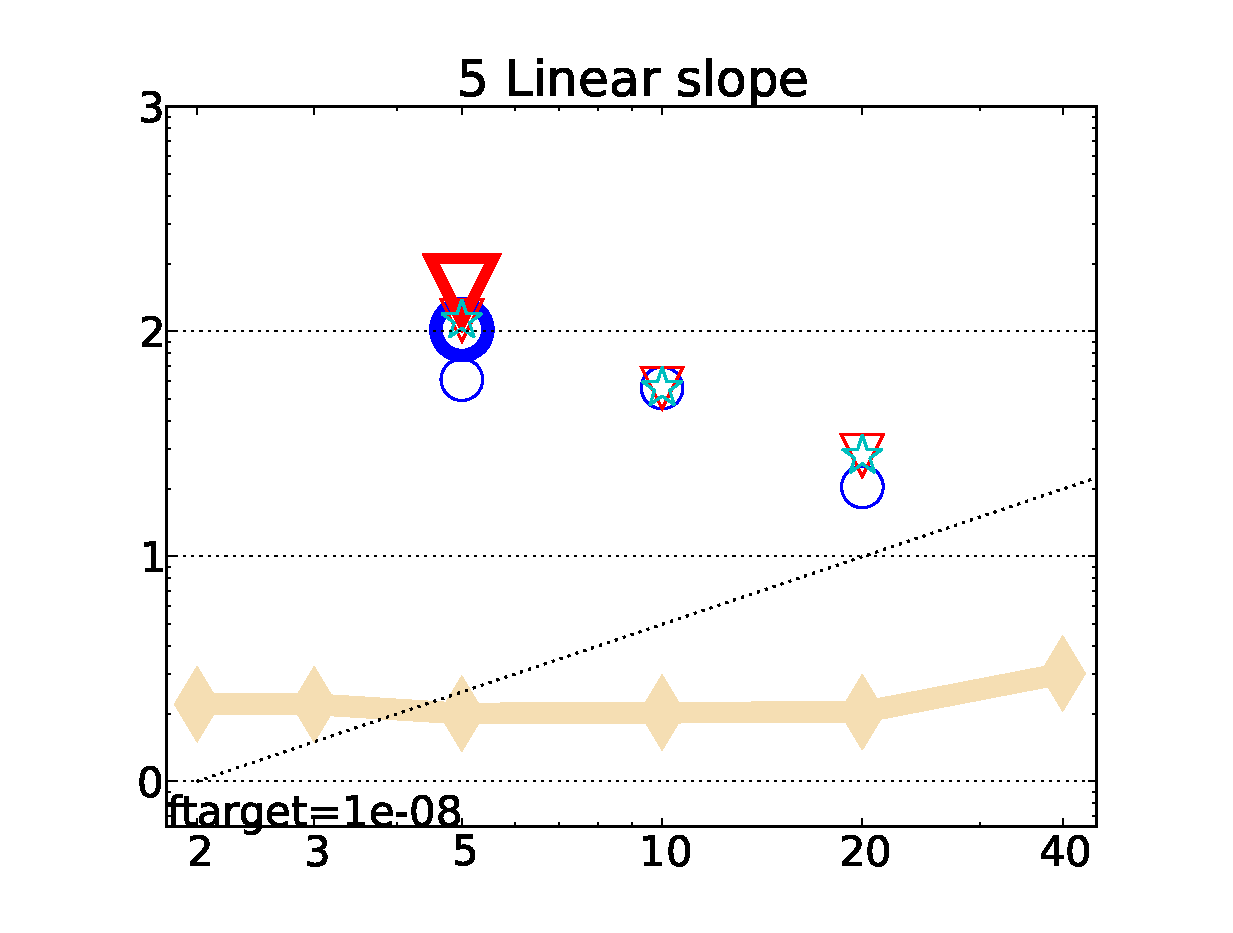
\includegraphics[width=0.25\textwidth, trim=20mm 7mm 15mm 3mm, clip]{ppfigs_f005}&
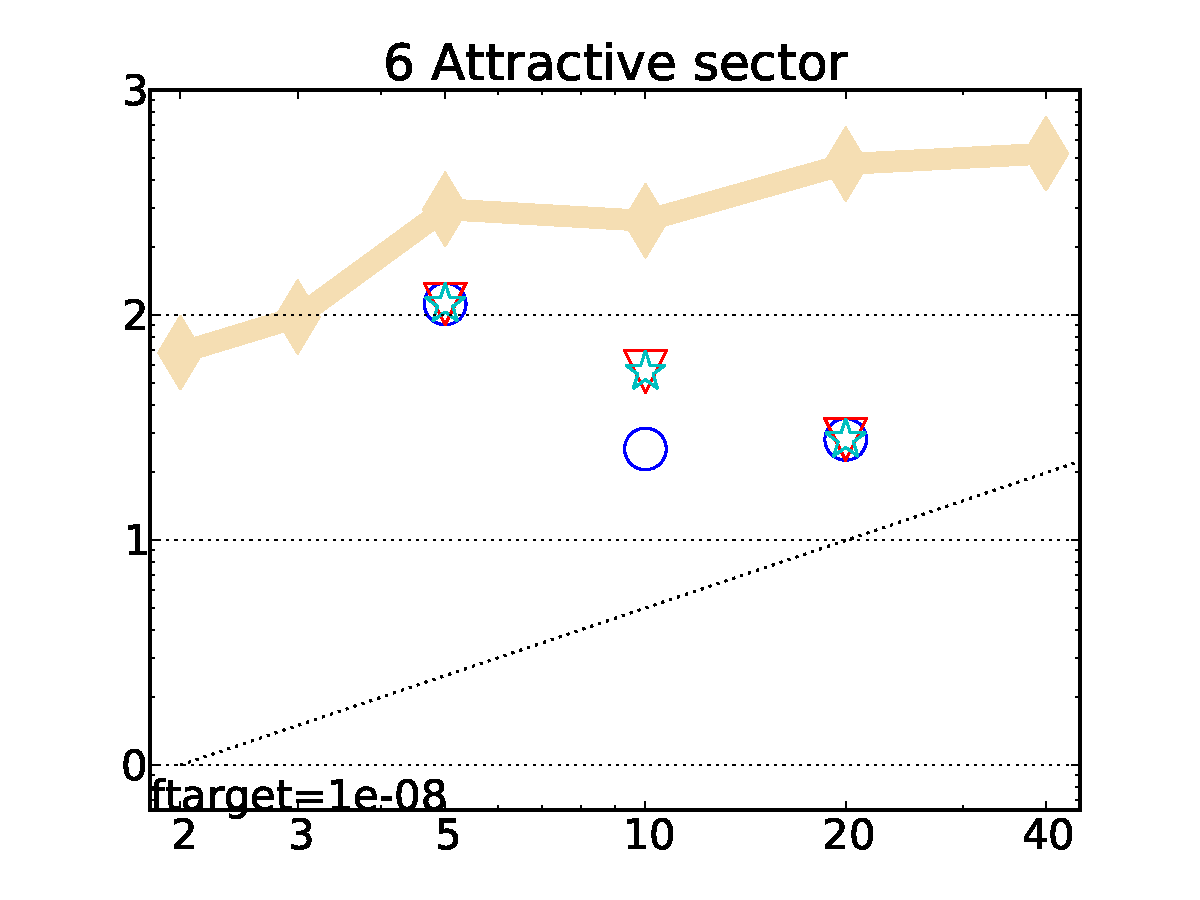
\includegraphics[width=0.25\textwidth, trim=20mm 7mm 15mm 3mm, clip]{ppfigs_f006}&
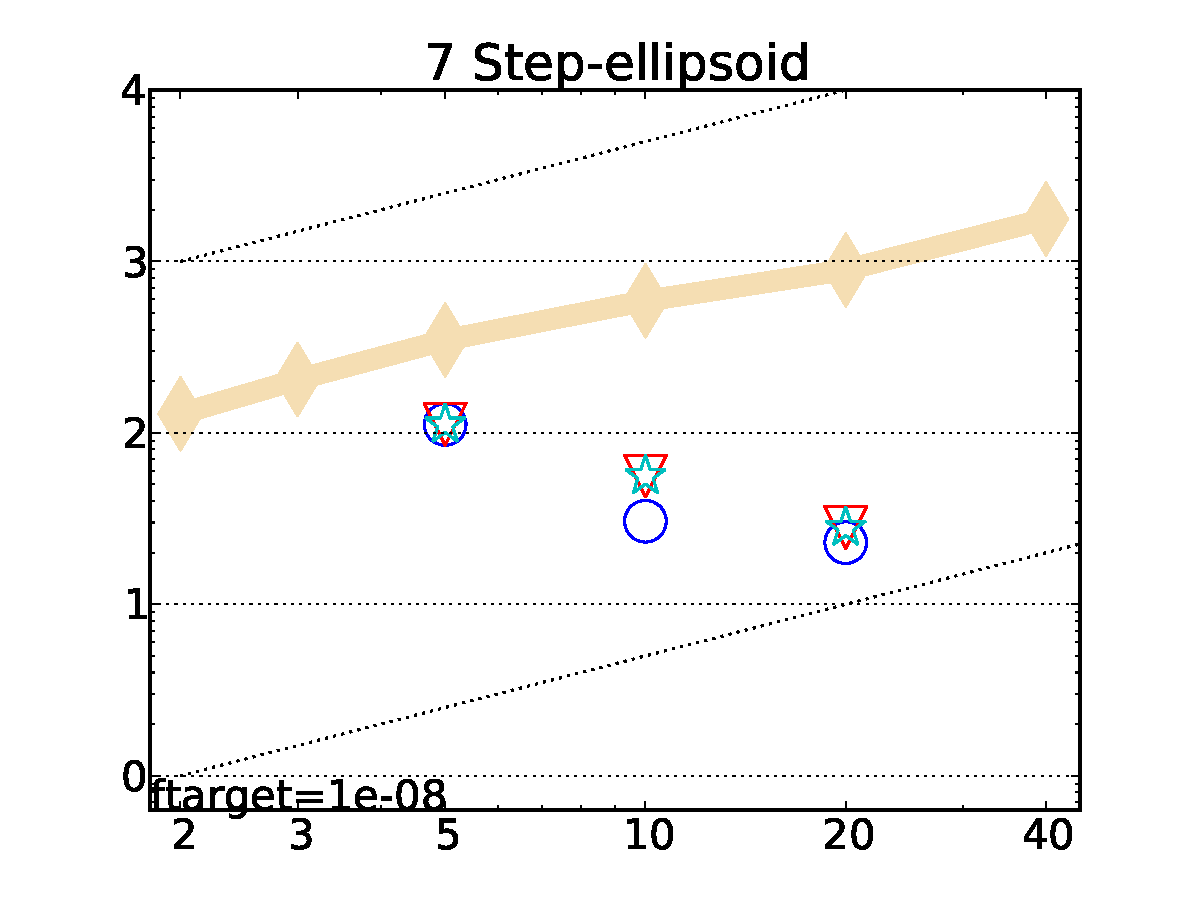
\includegraphics[width=0.25\textwidth, trim=20mm 7mm 15mm 3mm, clip]{ppfigs_f007}&
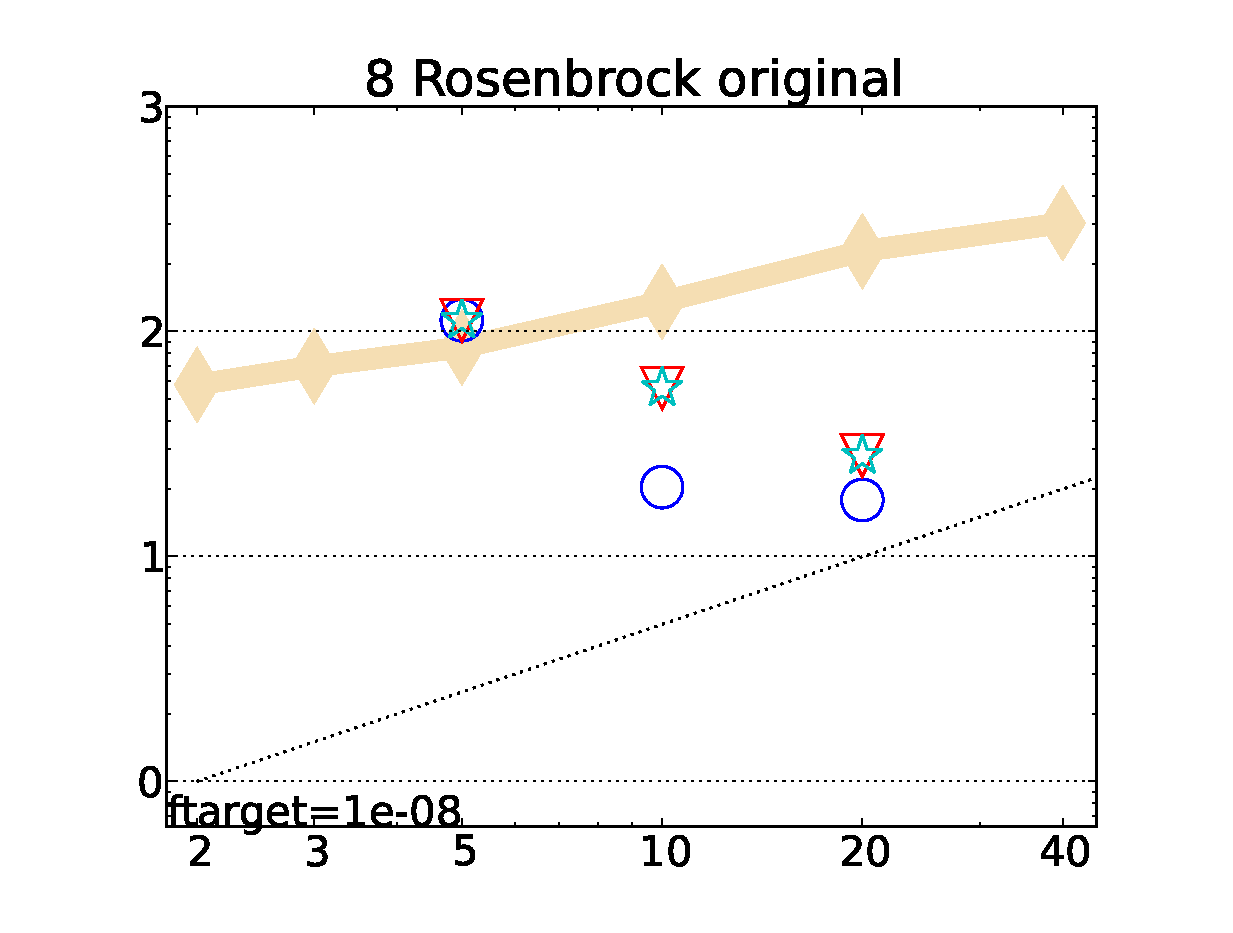
\includegraphics[width=0.25\textwidth, trim=20mm 7mm 15mm 3mm, clip]{ppfigs_f008}\\
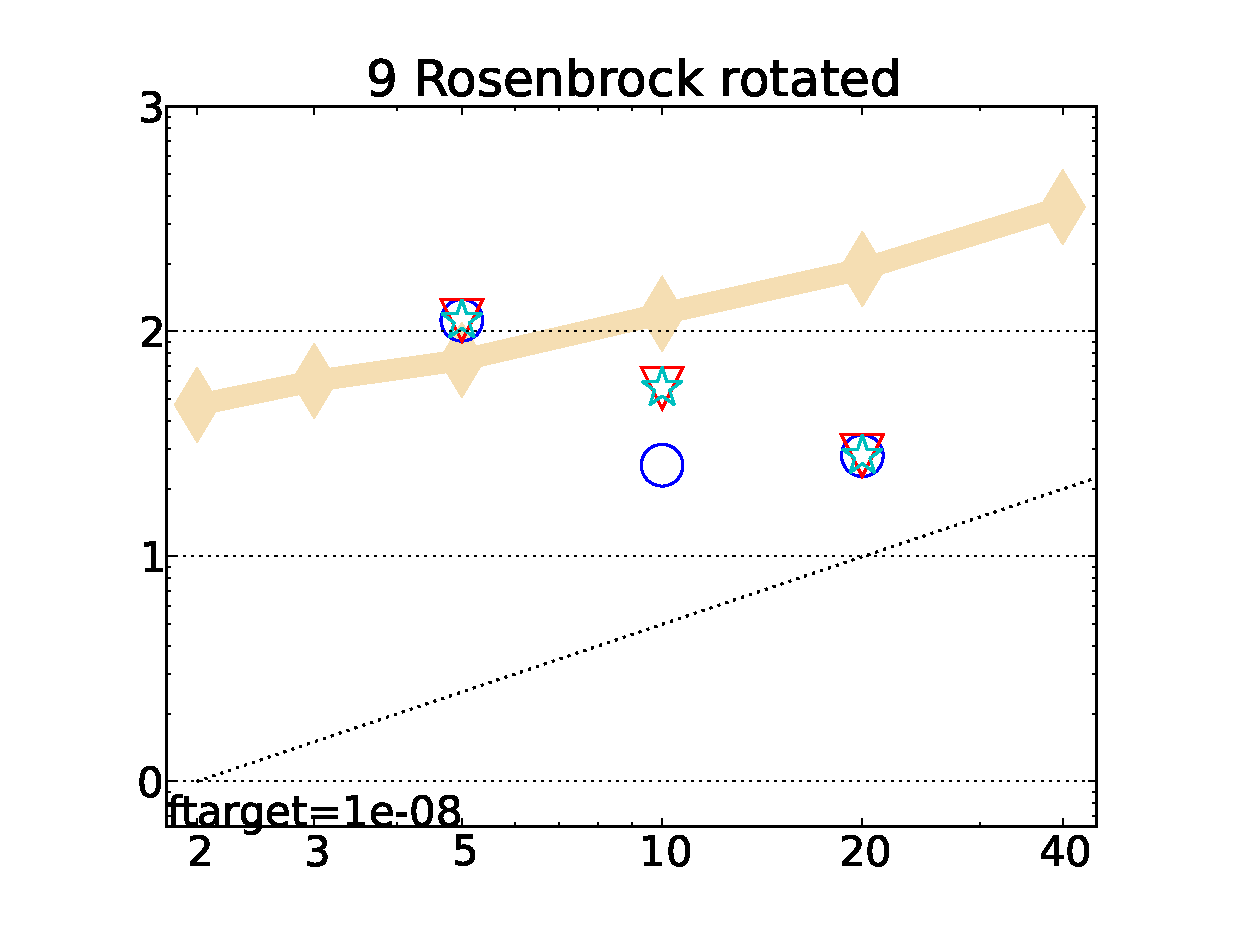
\includegraphics[width=0.25\textwidth, trim=20mm 7mm 15mm 3mm, clip]{ppfigs_f009}&
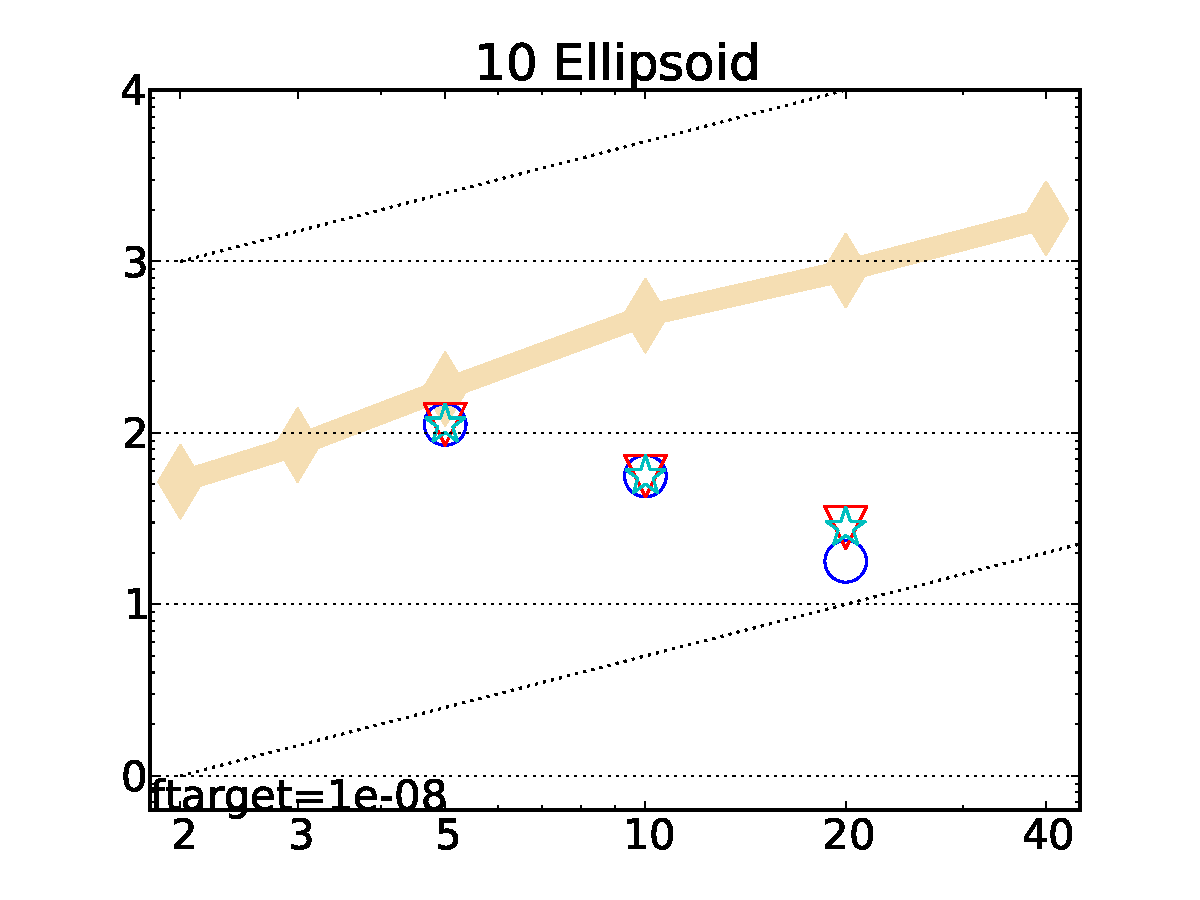
\includegraphics[width=0.25\textwidth, trim=20mm 7mm 15mm 3mm, clip]{ppfigs_f010}&
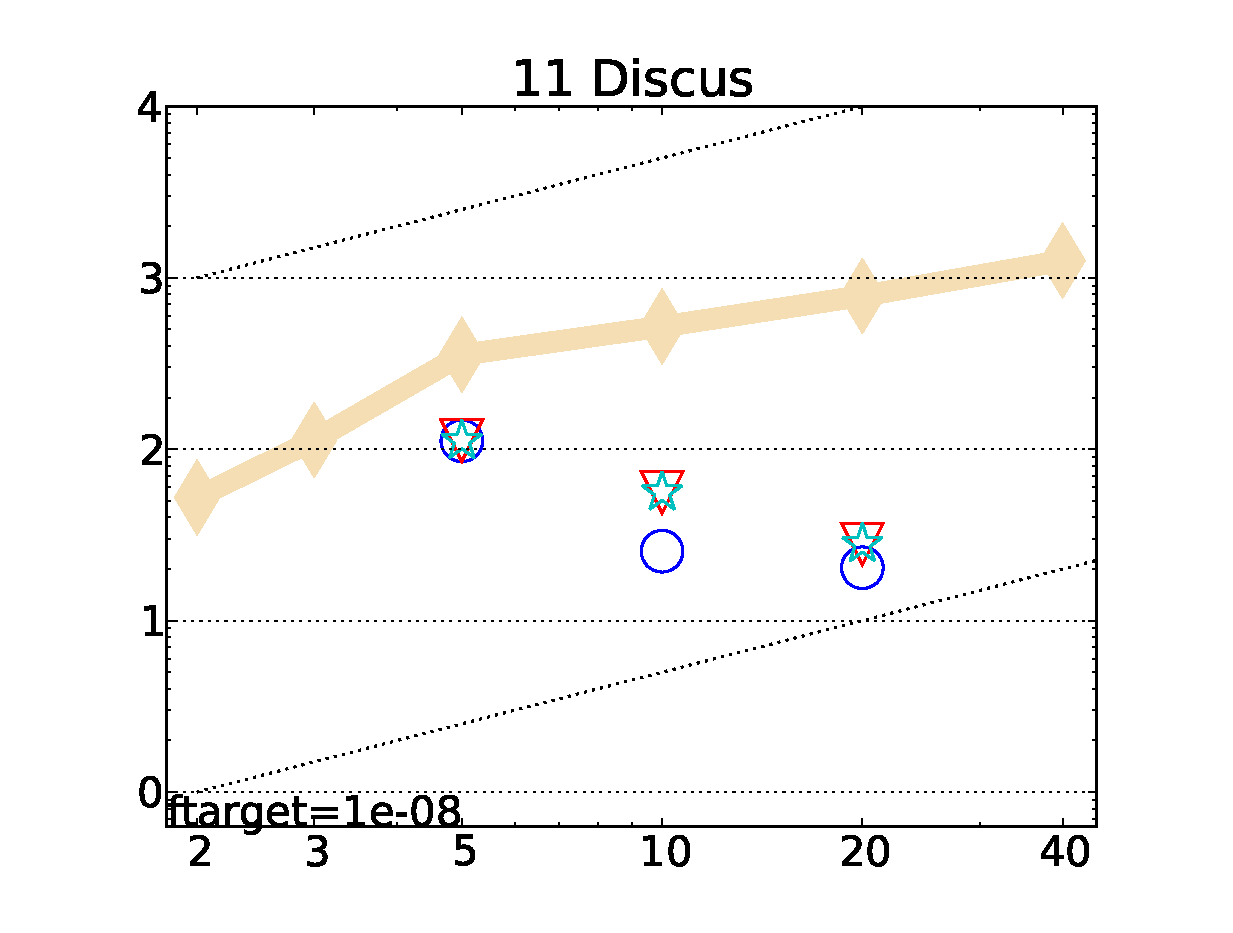
\includegraphics[width=0.25\textwidth, trim=20mm 7mm 15mm 3mm, clip]{ppfigs_f011}&
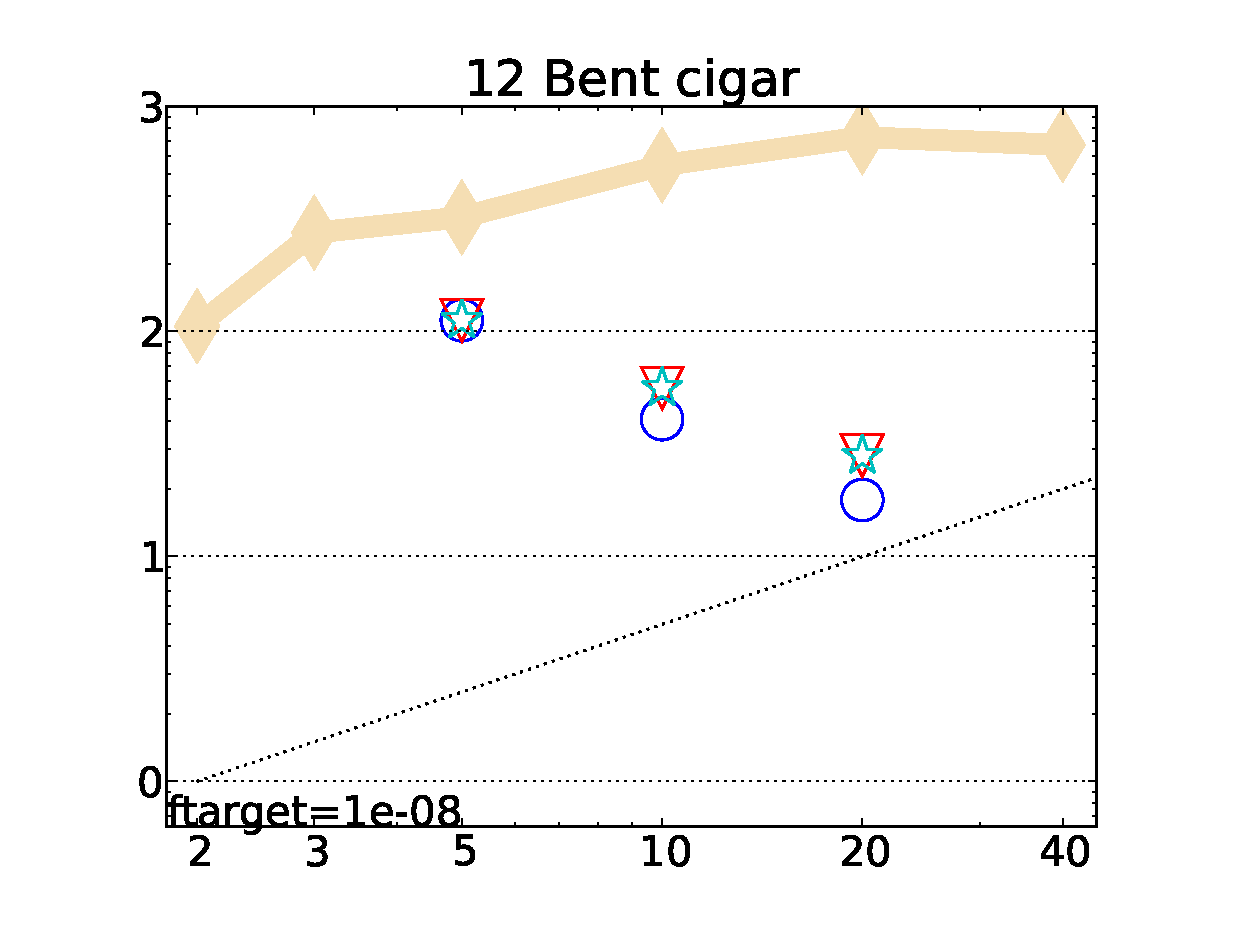
\includegraphics[width=0.25\textwidth, trim=20mm 7mm 15mm 3mm, clip]{ppfigs_f012}\\
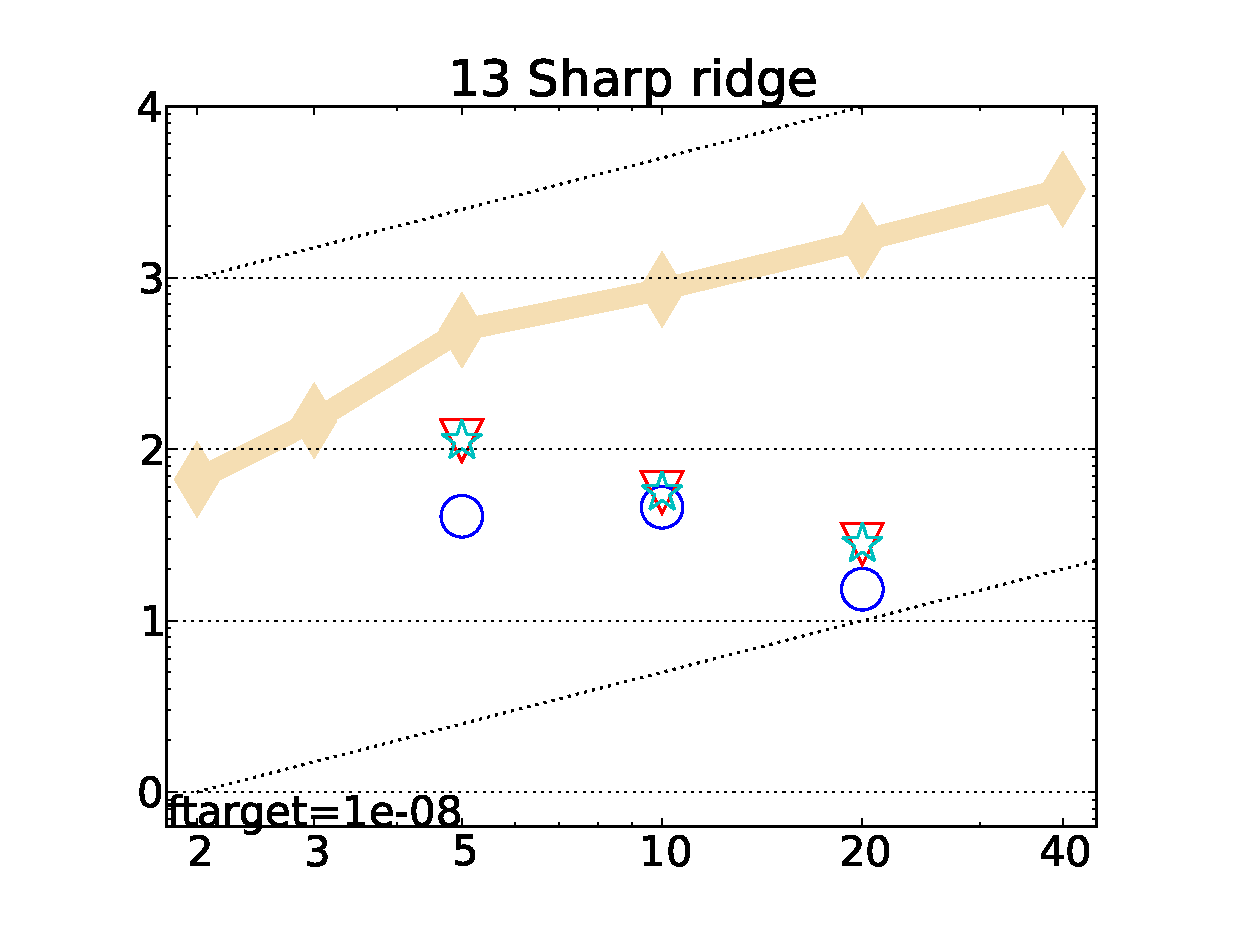
\includegraphics[width=0.25\textwidth, trim=20mm 7mm 15mm 3mm, clip]{ppfigs_f013}&
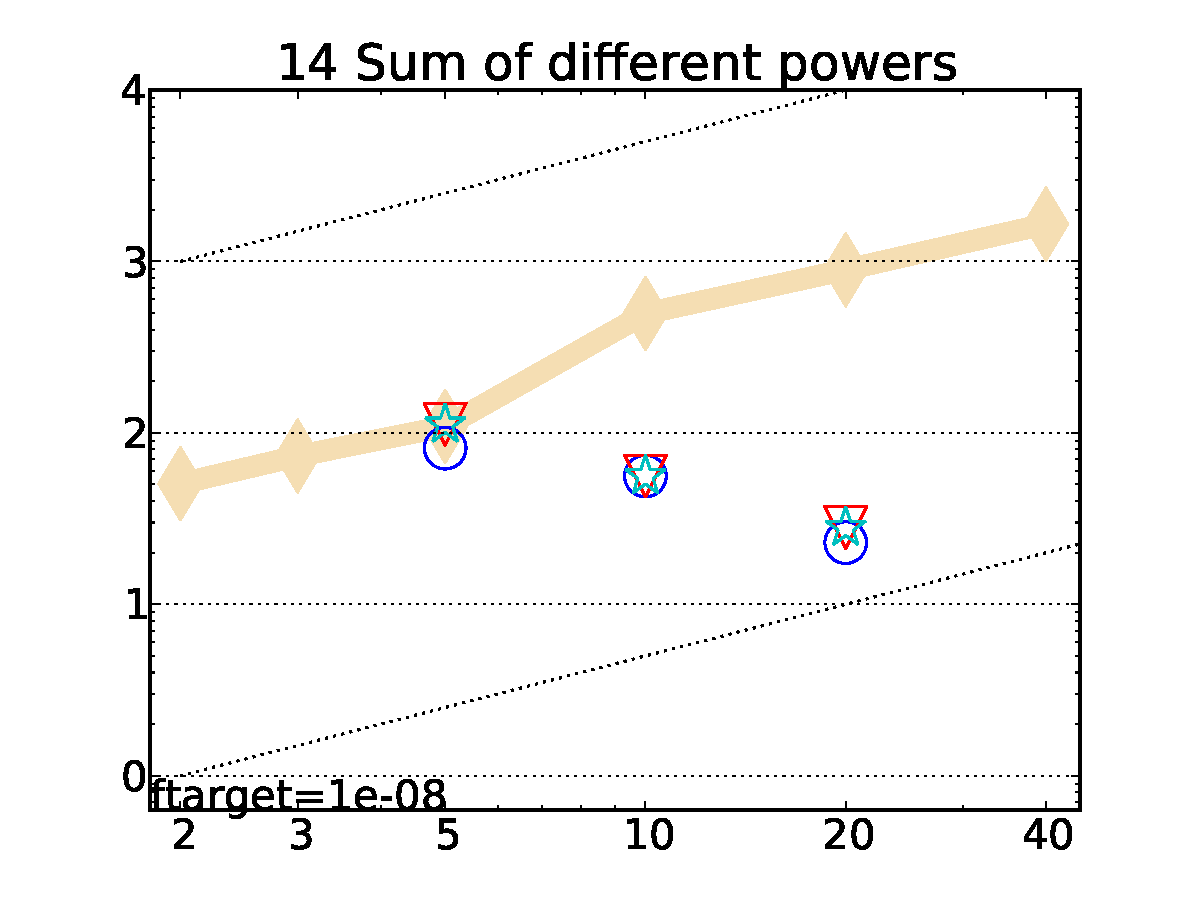
\includegraphics[width=0.25\textwidth, trim=20mm 7mm 15mm 3mm, clip]{ppfigs_f014}&
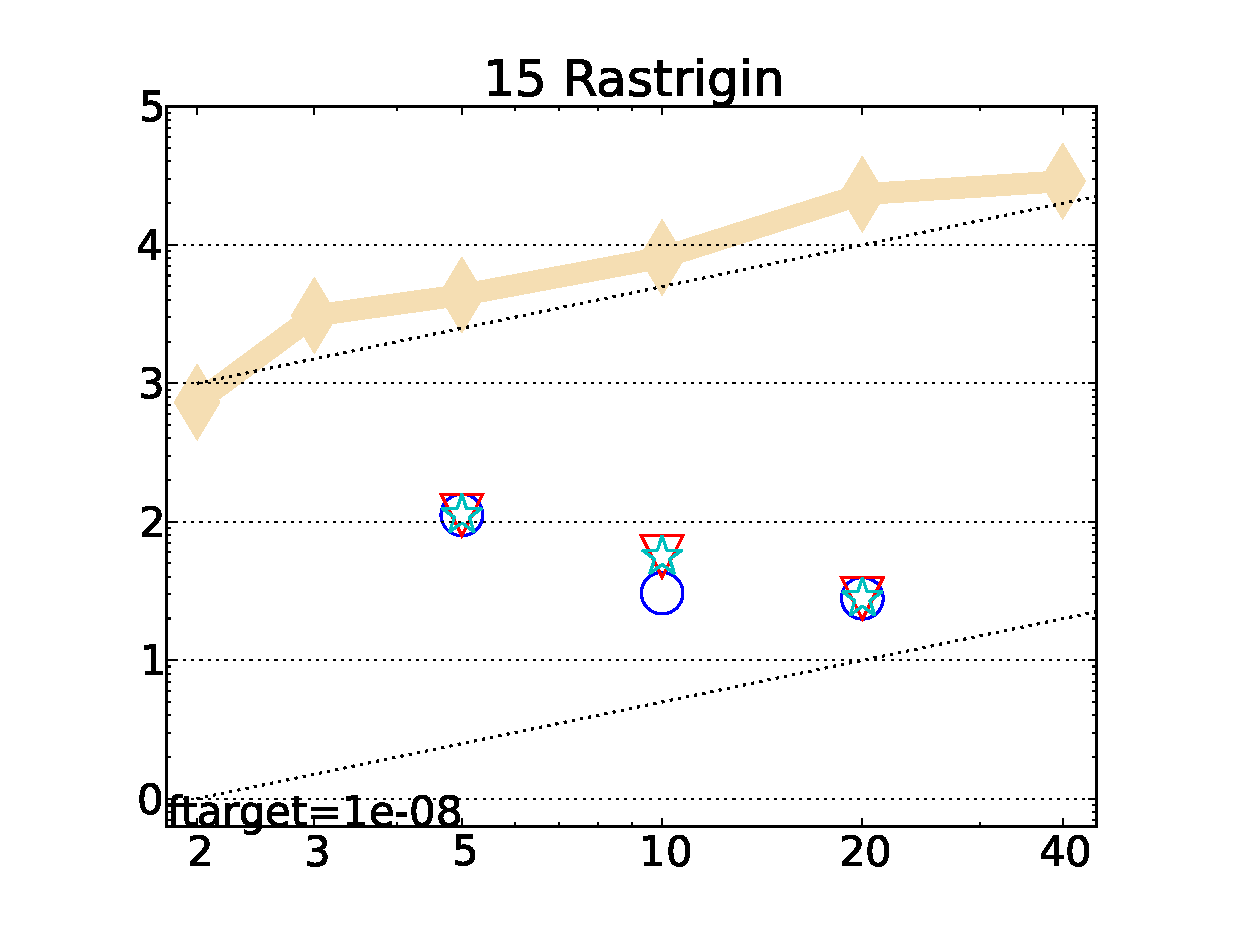
\includegraphics[width=0.25\textwidth, trim=20mm 7mm 15mm 3mm, clip]{ppfigs_f015}&
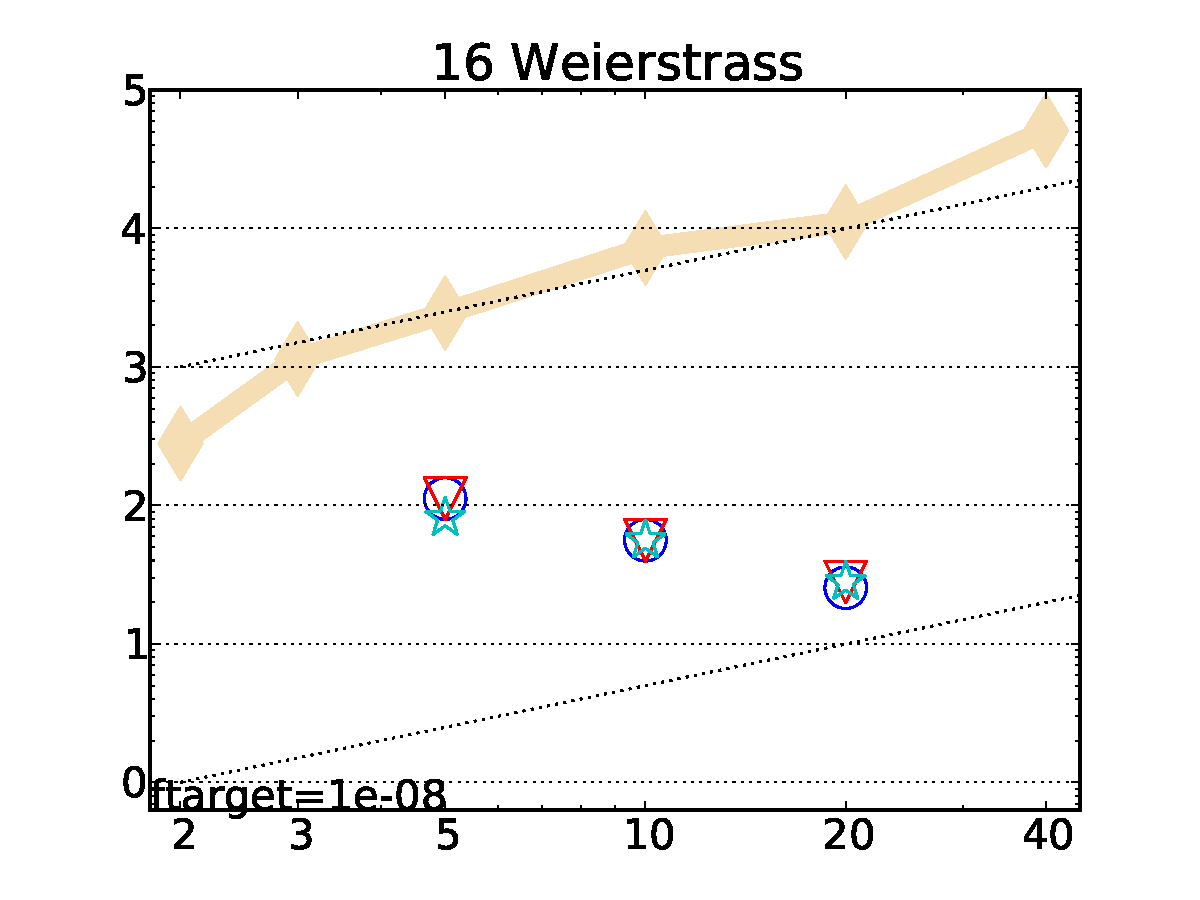
\includegraphics[width=0.25\textwidth, trim=20mm 7mm 15mm 3mm, clip]{ppfigs_f016}\\
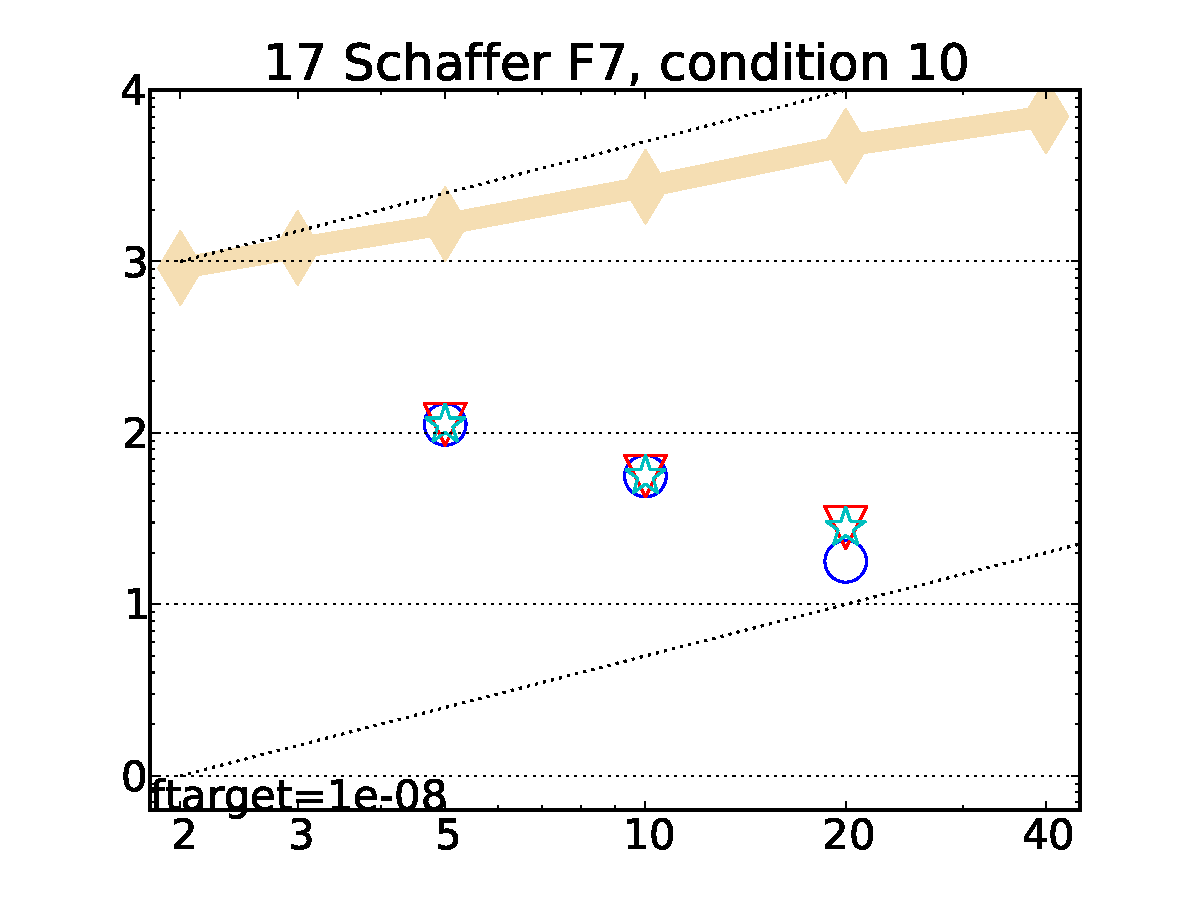
\includegraphics[width=0.25\textwidth, trim=20mm 7mm 15mm 3mm, clip]{ppfigs_f017}&
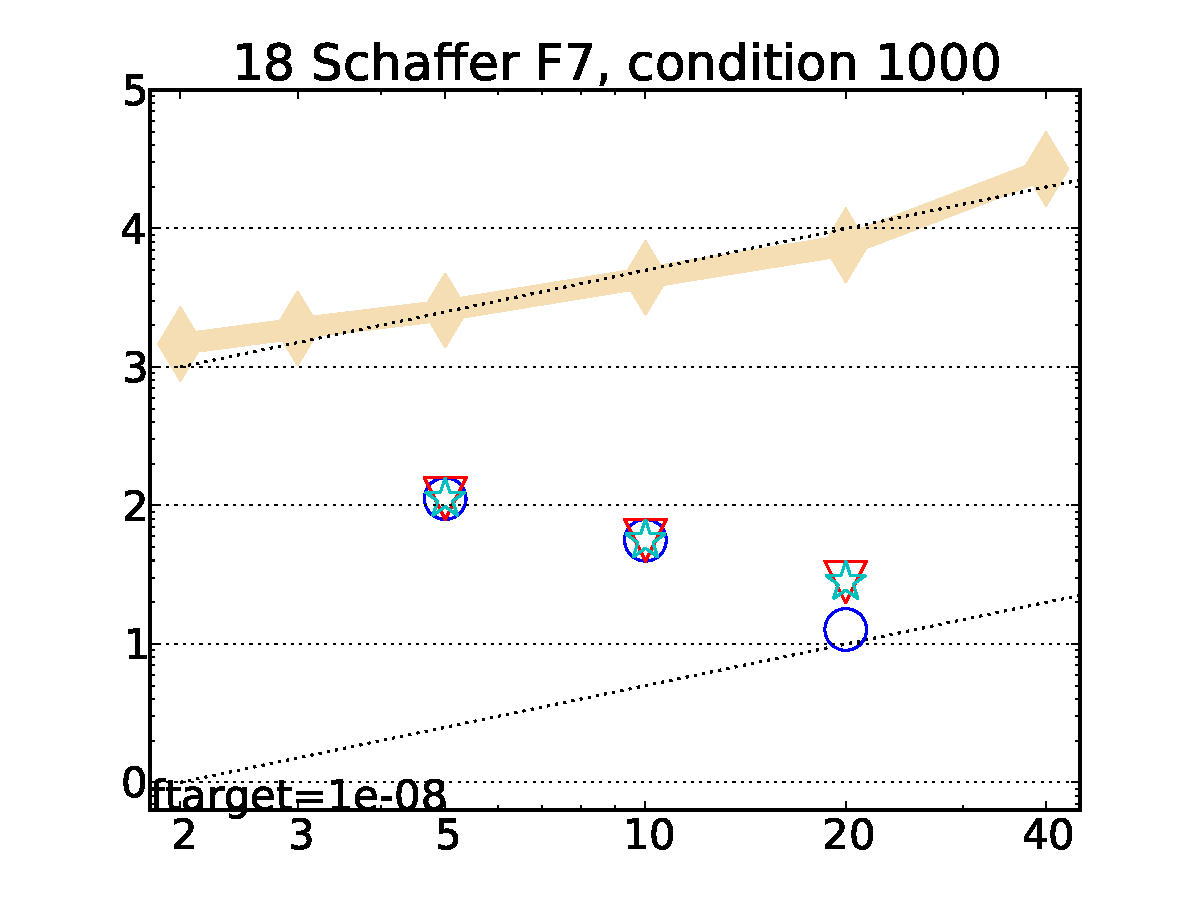
\includegraphics[width=0.25\textwidth, trim=20mm 7mm 15mm 3mm, clip]{ppfigs_f018}&
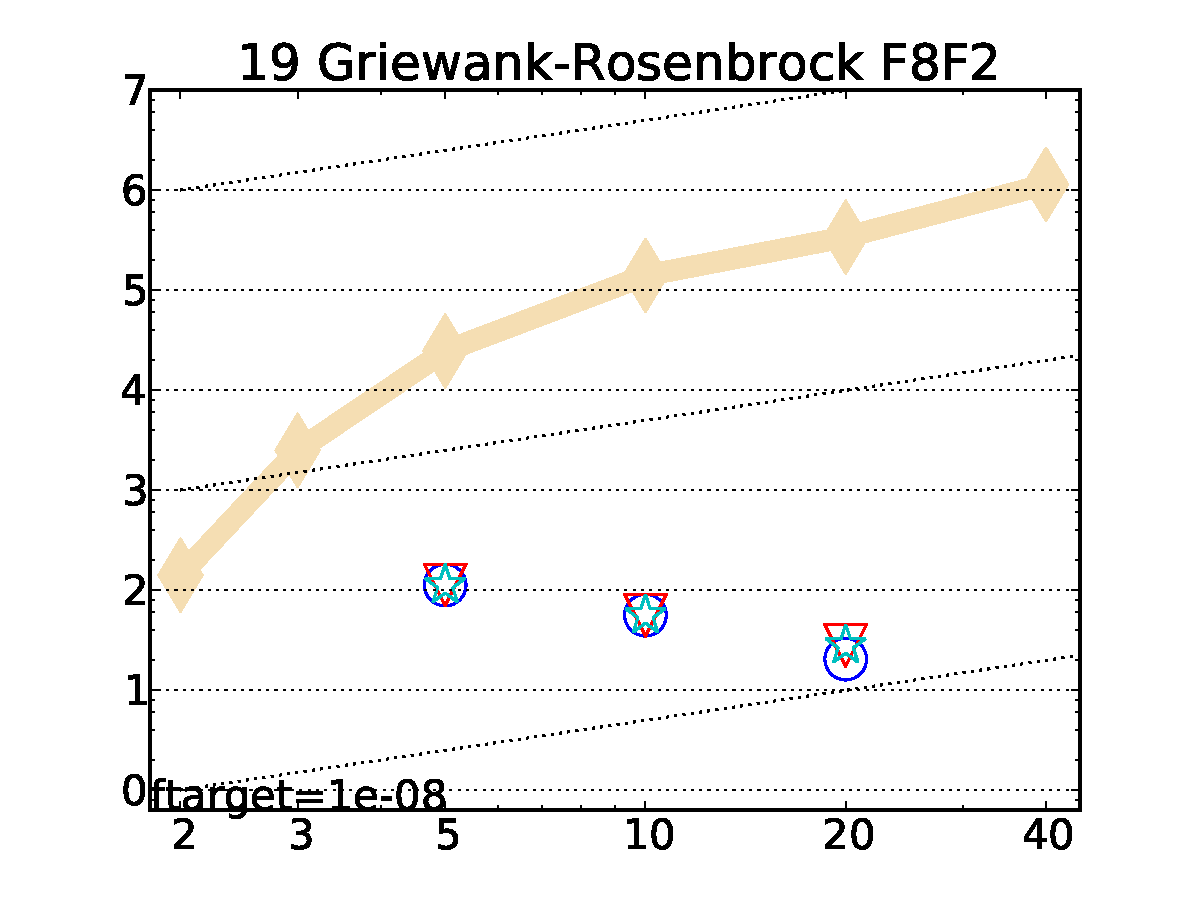
\includegraphics[width=0.25\textwidth, trim=20mm 7mm 15mm 3mm, clip]{ppfigs_f019}&
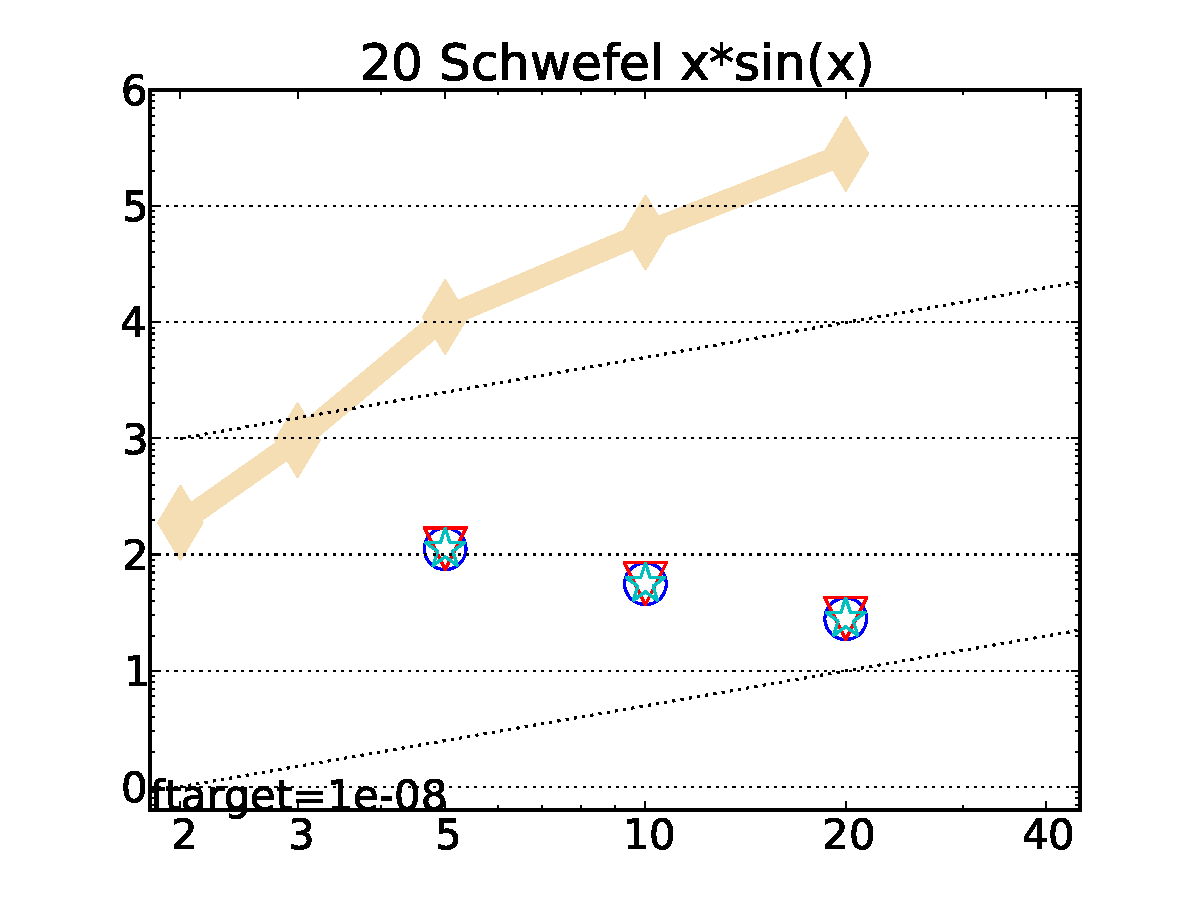
\includegraphics[width=0.25\textwidth, trim=20mm 7mm 15mm 3mm, clip]{ppfigs_f020}\\
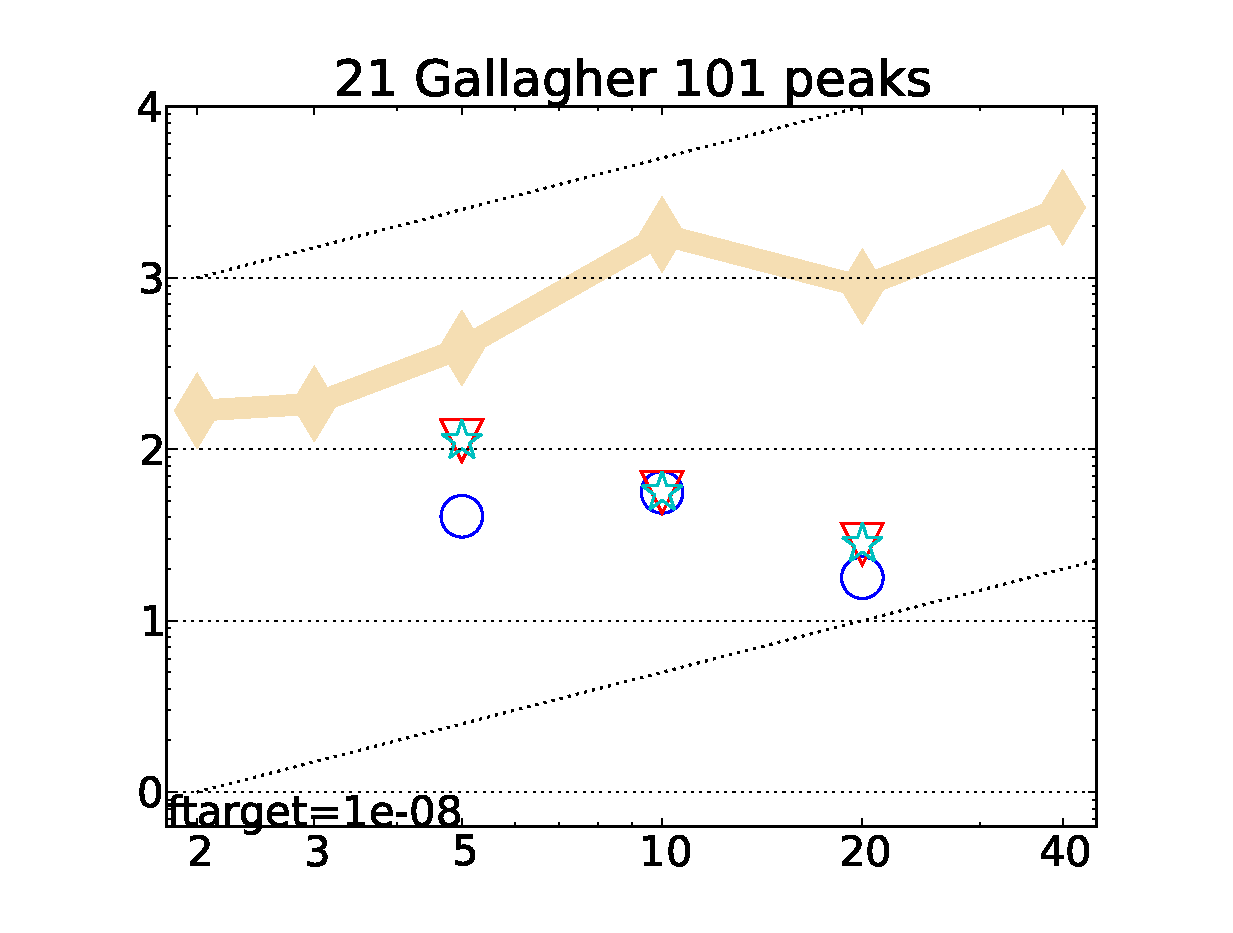
\includegraphics[width=0.25\textwidth, trim=20mm 7mm 15mm 3mm, clip]{ppfigs_f021}&
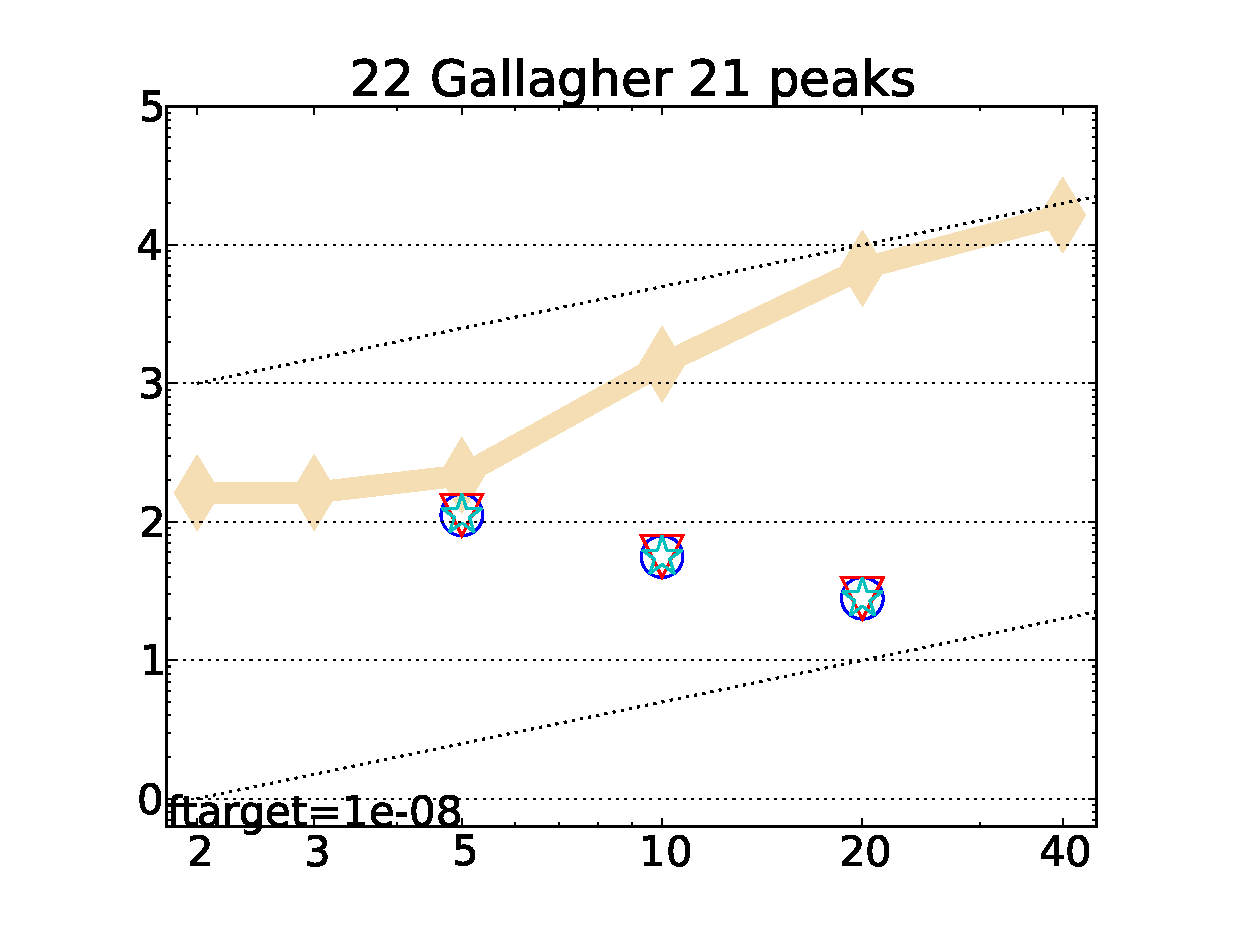
\includegraphics[width=0.25\textwidth, trim=20mm 7mm 15mm 3mm, clip]{ppfigs_f022}&
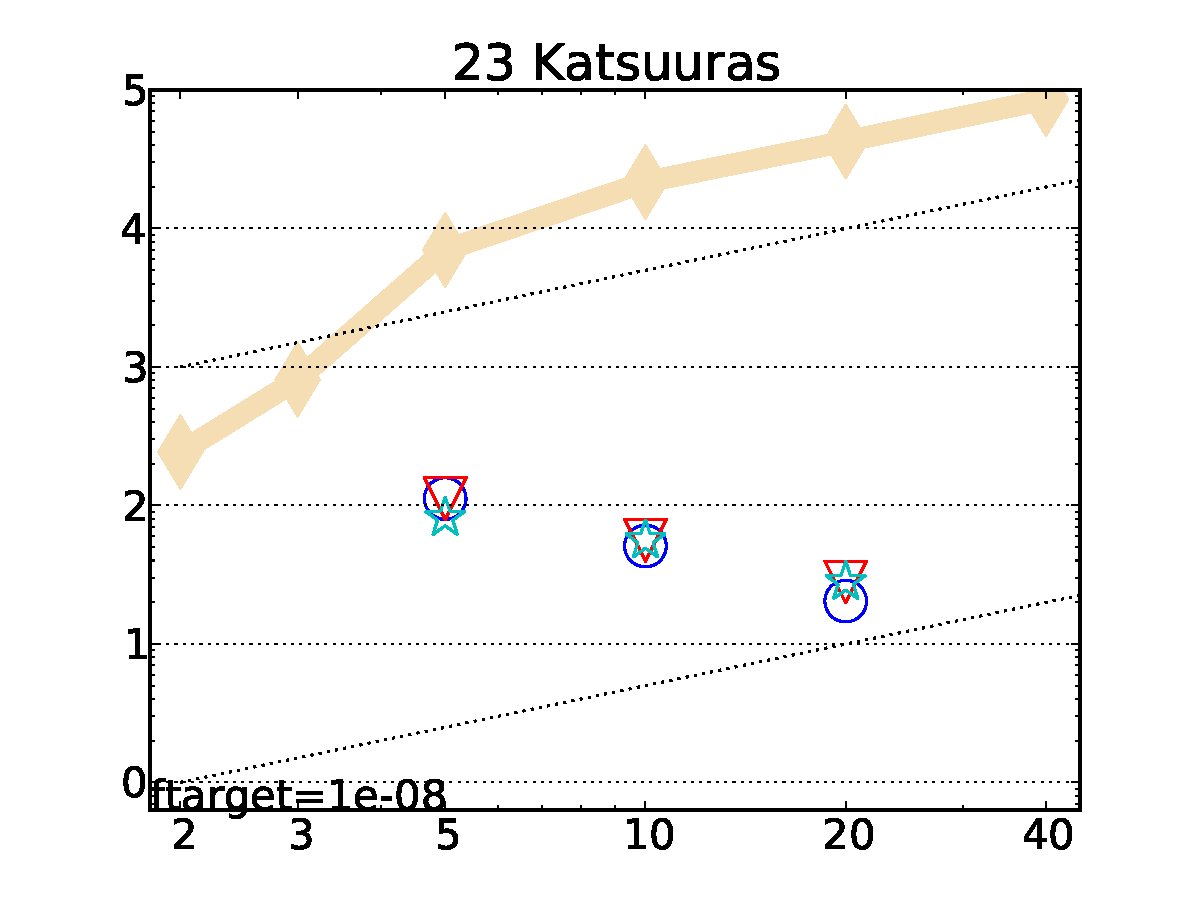
\includegraphics[width=0.25\textwidth, trim=20mm 7mm 15mm 3mm, clip]{ppfigs_f023}&
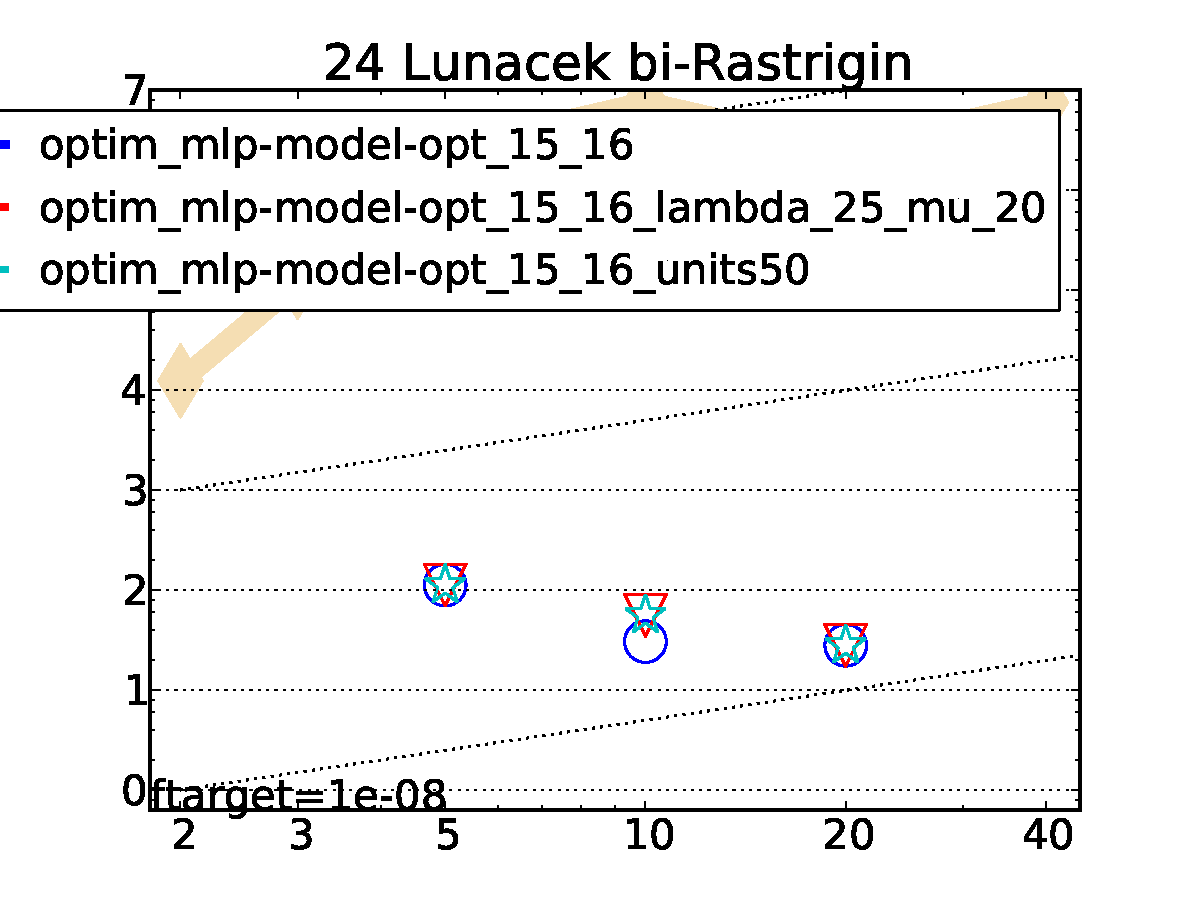
\includegraphics[width=0.25\textwidth, trim=20mm 7mm 15mm 3mm, clip]{ppfigs_f024}
\end{tabular}
\vspace*{-0.2cm}
\caption[Expected running time divided by dimension
versus dimension]{
\label{fig:scaling}
% command defined in bbob_pproc_commands.tex:
\bbobppfigslegend{$f_1$ and $f_{24}$}.  % \algorithmA can be defined above, see above
% Expected running time (\ERT) divided by dimension for target function value $10^{-8}$ as $\log_{10}$ values. Different symbols correspond to different algorithms given in legend of $f_1$ and $f_{24}$. Light symbols give the maximum number of function evaluations from all trials divided by the dimension. Horizontal lines give linear scaling, the slanted dotted lines give quadratic scaling.
% \input{\bbobdatapath ppfigs}
}
% The legend is in file \bbobdatapath ppfigs.tex
% While compiling this document, if the following error comes up:
% ! Undefined control sequence.
% try uncommenting line 9 and 10
\end{figure}
%%%%%%%%%%%%%%%%%%%%%%%%%%%%%%%%%%%%%%%%%%%%%%%%%%%%%%%%%%%%%%%%%%%%%%%%%%%%%%%
%%%%%%%%%%%%%%%%%%%%%%%%%%%%%%%%%%%%%%%%%%%%%%%%%%%%%%%%%%%%%%%%%%%%%%%%%%%%%%%
% The following line shows the figure as they are:
% \newcommand{\includeperfprof}[1]{\includegraphics[width=0.5\textwidth,trim=0mm 0mm 0mm 10mm, clip]{#1}}
% The following uncommented line clips the right of the figures and uses the
% information in file \bbobdatapath pprldmany_XXD_XXX.tex for displaying the
% right hand legend information, thus allowing to modify the algorithm names
% in the legend.
\newcommand{\includeperfprof}[1]{% include and annotate at the side
  \input{\bbobdatapath #1}%
  \includegraphics[width=0.4135\textwidth,trim=0mm 0mm 34mm 10mm, clip]{#1}%
  \raisebox{.037\textwidth}{\parbox[b][.3\textwidth]{.0868\textwidth}{\begin{scriptsize}
    \perfprofsidepanel % this is "\algaperfprof \vfill \algbperfprof \vfill" etc
  \end{scriptsize}}}
}
% Algorithm names on the right of the ECDF figures can be modified by
% uncommenting the following lines and inputting some text in the last
% brackets, make sure the algorithms are in the same order than for the post-processing:
% \newcommand{\algaperfprof}{Algorithm a short name}
% \newcommand{\algbperfprof}{Algorithm b short name}
% ...
% \newcommand{\algzperfprof}{Algorithm z short name}
% \newcommand{\algAperfprof}{Algorithm A short name}
% ...
%%%%%%%%%%%%%%%%%%%%%%%%%%%%%%%%%%%%%%%%%%%%%%%%%%%%%%%%%%%%%%%%%%%%%%%%%%%%%%%
%%%%%%%%%%%%%%%%%%%%%%%%%%%%%%%%%%%%%%%%%%%%%%%%%%%%%%%%%%%%%%%%%%%%%%%%%%%%%%%
\begin{figure}
 \begin{tabular}{@{}c@{}c@{}}
 separable fcts & moderate fcts \\
 \includeperfprof{pprldmany_05D_separ} &
 \includeperfprof{pprldmany_05D_lcond} \\ 
ill-conditioned fcts & multi-modal fcts \\
 \includeperfprof{pprldmany_05D_hcond} &
 \includeperfprof{pprldmany_05D_multi} \\ 
 weakly structured multi-modal fcts & all functions\\
 \includeperfprof{pprldmany_05D_mult2} & 
 \includeperfprof{pprldmany_05D_noiselessall} 
 \end{tabular}
\caption{\label{fig:ECDFs05D}
Bootstrapped empirical cumulative distribution of 
the number of objective function evaluations
% \# of $f$-evaluations 
divided by dimension for 50 targets in
$10^{[-8..2]}$ for all functions and subgroups in 5-D. The ``best 2009'' line
corresponds to the best \ERT\ observed during BBOB 2009 for each single target. 
}
\end{figure}
%%%%%%%%%%%%%%%%%%%%%%%%%%%%%%%%%%%%%%%%%%%%%%%%%%%%%%%%%%%%%%%%%%%%%%%%%%%%%%%
%%%%%%%%%%%%%%%%%%%%%%%%%%%%%%%%%%%%%%%%%%%%%%%%%%%%%%%%%%%%%%%%%%%%%%%%%%%%%%%
\begin{figure}
 \begin{tabular}{@{}c@{}c@{}}
 separable fcts & moderate fcts \\
 \includeperfprof{pprldmany_20D_separ} &
 \includeperfprof{pprldmany_20D_lcond} \\ 
ill-conditioned fcts & multi-modal fcts \\
 \includeperfprof{pprldmany_20D_hcond} &
 \includeperfprof{pprldmany_20D_multi} \\ 
 weakly structured multi-modal fcts & all functions\\
 \includeperfprof{pprldmany_20D_mult2} & 
 \includeperfprof{pprldmany_20D_noiselessall} 
 \end{tabular}
\caption{
\label{fig:ECDFs20D}
Bootstrapped empirical cumulative distribution of 
the number of objective function evaluations
% \# of $f$-evaluations 
divided by dimension for 50 targets in
$10^{[-8..2]}$ for all functions and subgroups in 20-D. The ``best 2009'' line
corresponds to the best \ERT\ observed during BBOB 2009 for each single target. 
}
\end{figure}
%%%%%%%%%%%%%%%%%%%%%%%%%%%%%%%%%%%%%%%%%%%%%%%%%%%%%%%%%%%%%%%%%%%%%%%%%%%%%%%
%%%%%%%%%%%%%%%%%%%%%%%%%%%%%%%%%%%%%%%%%%%%%%%%%%%%%%%%%%%%%%%%%%%%%%%%%%%%%%%
% Algorithm names in the tables can be modified by uncommenting the following
% lines and inputting some text in the last brackets, make sure the algorithms
% are in the same order than for the post-processing:
% \newcommand{\algatables}{Algorithm a short name}
% \newcommand{\algbtables}{Algorithm b short name}
% ...
% \newcommand{\algztables}{Algorithm z short name}
% \newcommand{\algAtables}{Algorithm A short name}
% ...
%%%%%%%%%%%%%%%%%%%%%%%%%%%%%%%%%%%%%%%%%%%%%%%%%%%%%%%%%%%%%%%%%%%%%%%%%%%%%%%
%%%%%%%%%%%%%%%%%%%%%%%%%%%%%%%%%%%%%%%%%%%%%%%%%%%%%%%%%%%%%%%%%%%%%%%%%%%%%%%
\clearpage
\begin{table}
\caption{\label{tab:f1_05D}\tablecaption{1}{5}}
\centering
\footnotesize
\input{\bbobdatapath pptables_f001_05D}
\end{table}
\begin{table}
\caption{\label{tab:f2_05D}\tablecaption{2}{5}}
\centering
\footnotesize
\input{\bbobdatapath pptables_f002_05D}
\end{table}
\begin{table}
\caption{\label{tab:f3_05D}\tablecaption{3}{5}}
\centering
\footnotesize
\input{\bbobdatapath pptables_f003_05D}
\end{table}
\begin{table}
\caption{\label{tab:f4_05D}\tablecaption{4}{5}}
\centering
\footnotesize
\input{\bbobdatapath pptables_f004_05D}
\end{table}
\begin{table}
\caption{\label{tab:f5_05D}\tablecaption{5}{5}}
\centering
\footnotesize
\input{\bbobdatapath pptables_f005_05D}
\end{table}
\begin{table}
\caption{\label{tab:f6_05D}\tablecaption{6}{5}}
\centering
\footnotesize
\input{\bbobdatapath pptables_f006_05D}
\end{table}
\begin{table}
\caption{\label{tab:f7_05D}\tablecaption{7}{5}}
\centering
\footnotesize
\input{\bbobdatapath pptables_f007_05D}
\end{table}
\begin{table}
\caption{\label{tab:f8_05D}\tablecaption{8}{5}}
\centering
\footnotesize
\input{\bbobdatapath pptables_f008_05D}
\end{table}
\begin{table}
\caption{\label{tab:f9_05D}\tablecaption{9}{5}}
\centering
\footnotesize
\input{\bbobdatapath pptables_f009_05D}
\end{table}
\begin{table}
\caption{\label{tab:f10_05D}\tablecaption{10}{5}}
\centering
\footnotesize
\input{\bbobdatapath pptables_f010_05D}
\end{table}
\begin{table}
\caption{\label{tab:f11_05D}\tablecaption{11}{5}}
\centering
\footnotesize
\input{\bbobdatapath pptables_f011_05D}
\end{table}
\begin{table}
\caption{\label{tab:f12_05D}\tablecaption{12}{5}}
\centering
\footnotesize
\input{\bbobdatapath pptables_f012_05D}
\end{table}
\clearpage
\begin{table}
\caption{\label{tab:f13_05D}\tablecaption{13}{5}}
\centering
\footnotesize
\input{\bbobdatapath pptables_f013_05D}
\end{table}
\begin{table}
\caption{\label{tab:f14_05D}\tablecaption{14}{5}}
\centering
\footnotesize
\input{\bbobdatapath pptables_f014_05D}
\end{table}
\begin{table}
\caption{\label{tab:f15_05D}\tablecaption{15}{5}}
\centering
\footnotesize
\input{\bbobdatapath pptables_f015_05D}
\end{table}
\begin{table}
\caption{\label{tab:f16_05D}\tablecaption{16}{5}}
\centering
\footnotesize
\input{\bbobdatapath pptables_f016_05D}
\end{table}
\begin{table}
\caption{\label{tab:f17_05D}\tablecaption{17}{5}}
\centering
\footnotesize
\input{\bbobdatapath pptables_f017_05D}
\end{table}
\begin{table}
\caption{\label{tab:f18_05D}\tablecaption{18}{5}}
\centering
\footnotesize
\input{\bbobdatapath pptables_f018_05D}
\end{table}
\begin{table}
\caption{\label{tab:f19_05D}\tablecaption{19}{5}}
\centering
\footnotesize
\input{\bbobdatapath pptables_f019_05D}
\end{table}
\begin{table}
\caption{\label{tab:f20_05D}\tablecaption{20}{5}}
\centering
\footnotesize
\input{\bbobdatapath pptables_f020_05D}
\end{table}
\begin{table}
\caption{\label{tab:f21_05D}\tablecaption{21}{5}}
\centering
\footnotesize
\input{\bbobdatapath pptables_f021_05D}
\end{table}
\begin{table}
\caption{\label{tab:f22_05D}\tablecaption{22}{5}}
\centering
\footnotesize
\input{\bbobdatapath pptables_f022_05D}
\end{table}
\begin{table}
\caption{\label{tab:f23_05D}\tablecaption{23}{5}}
\centering
\footnotesize
\input{\bbobdatapath pptables_f023_05D}
\end{table}
\begin{table}
\caption{\label{tab:f24_05D}\tablecaption{24}{5}}
\centering
\footnotesize
\input{\bbobdatapath pptables_f024_05D}
\end{table}
%%%%%%%%%%%%%%%%%%%%%%%%%%%%%%%%%%%%%%%%%%%%%%%%%%%%%%%%%%%%%%%%%%%%%%%%%%%%%%%
%%%%%%%%%%%%%%%%%%%%%%%%%%%%%%%%%%%%%%%%%%%%%%%%%%%%%%%%%%%%%%%%%%%%%%%%%%%%%%%
\clearpage
\begin{table}
\caption{\label{tab:f1_20D}\tablecaption{1}{20}}
\centering
\footnotesize
\input{\bbobdatapath pptables_f001_20D}
\end{table}
\begin{table}
\caption{\label{tab:f2_20D}\tablecaption{2}{20}}
\centering
\footnotesize
\input{\bbobdatapath pptables_f002_20D}
\end{table}
\begin{table}
\caption{\label{tab:f3_20D}\tablecaption{3}{20}}
\centering
\footnotesize
\input{\bbobdatapath pptables_f003_20D}
\end{table}
\begin{table}
\caption{\label{tab:f4_20D}\tablecaption{4}{20}}
\centering
\footnotesize
\input{\bbobdatapath pptables_f004_20D}
\end{table}
\begin{table}
\caption{\label{tab:f5_20D}\tablecaption{5}{20}}
\centering
\footnotesize
\input{\bbobdatapath pptables_f005_20D}
\end{table}
\begin{table}
\caption{\label{tab:f6_20D}\tablecaption{6}{20}}
\centering
\footnotesize
\input{\bbobdatapath pptables_f006_20D}
\end{table}
\begin{table}
\caption{\label{tab:f7_20D}\tablecaption{7}{20}}
\centering
\footnotesize
\input{\bbobdatapath pptables_f007_20D}
\end{table}
\begin{table}
\caption{\label{tab:f8_20D}\tablecaption{8}{20}}
\centering
\footnotesize
\input{\bbobdatapath pptables_f008_20D}
\end{table}
\begin{table}
\caption{\label{tab:f9_20D}\tablecaption{9}{20}}
\centering
\footnotesize
\input{\bbobdatapath pptables_f009_20D}
\end{table}
\begin{table}
\caption{\label{tab:f10_20D}\tablecaption{10}{20}}
\centering
\footnotesize
\input{\bbobdatapath pptables_f010_20D}
\end{table}
\begin{table}
\caption{\label{tab:f11_20D}\tablecaption{11}{20}}
\centering
\footnotesize
\input{\bbobdatapath pptables_f011_20D}
\end{table}
\begin{table}
\caption{\label{tab:f12_20D}\tablecaption{12}{20}}
\centering
\footnotesize
\input{\bbobdatapath pptables_f012_20D}
\end{table}
\clearpage
\begin{table}
\caption{\label{tab:f13_20D}\tablecaption{13}{20}}
\centering
\footnotesize
\input{\bbobdatapath pptables_f013_20D}
\end{table}
\begin{table}
\caption{\label{tab:f14_20D}\tablecaption{14}{20}}
\centering
\footnotesize
\input{\bbobdatapath pptables_f014_20D}
\end{table}
\begin{table}
\caption{\label{tab:f15_20D}\tablecaption{15}{20}}
\centering
\footnotesize
\input{\bbobdatapath pptables_f015_20D}
\end{table}
\begin{table}
\caption{\label{tab:f16_20D}\tablecaption{16}{20}}
\centering
\footnotesize
\input{\bbobdatapath pptables_f016_20D}
\end{table}
\begin{table}
\caption{\label{tab:f17_20D}\tablecaption{17}{20}}
\centering
\footnotesize
\input{\bbobdatapath pptables_f017_20D}
\end{table}
\begin{table}
\caption{\label{tab:f18_20D}\tablecaption{18}{20}}
\centering
\footnotesize
\input{\bbobdatapath pptables_f018_20D}
\end{table}
\begin{table}
\caption{\label{tab:f19_20D}\tablecaption{19}{20}}
\centering
\footnotesize
\input{\bbobdatapath pptables_f019_20D}
\end{table}
\begin{table}
\caption{\label{tab:f20_20D}\tablecaption{20}{20}}
\centering
\footnotesize
\input{\bbobdatapath pptables_f020_20D}
\end{table}
\begin{table}
\caption{\label{tab:f21_20D}\tablecaption{21}{20}}
\centering
\footnotesize
\input{\bbobdatapath pptables_f021_20D}
\end{table}
\begin{table}
\caption{\label{tab:f22_20D}\tablecaption{22}{20}}
\centering
\footnotesize
\input{\bbobdatapath pptables_f022_20D}
\end{table}
\begin{table}
\caption{\label{tab:f23_20D}\tablecaption{23}{20}}
\centering
\footnotesize
\input{\bbobdatapath pptables_f023_20D}
\end{table}
\begin{table}
\caption{\label{tab:f24_20D}\tablecaption{24}{20}}
\centering
\footnotesize
\input{\bbobdatapath pptables_f024_20D}
\end{table}
%%%%%%%%%%%%%%%%%%%%%%%%%%%%%%%%%%%%%%%%%%%%%%%%%%%%%%%%%%%%%%%%%%%%%%%%%%%%%%%
%%%%%%%%%%%%%%%%%%%%%%%%%%%%%%%%%%%%%%%%%%%%%%%%%%%%%%%%%%%%%%%%%%%%%%%%%%%%%%%
% The following two commands are all you need in the
% initial runs of your .tex file to
% produce the bibliography for the citations in your paper.
\bibliographystyle{abbrv}
\bibliography{bbob}  % bbob.bib is the name of the Bibliography in this case
% You must have a proper ".bib" file
%  and remember to run:
% latex bibtex latex latex
% to resolve all references
\end{document}

